\documentclass[journal]{IEEEtran}

\input{stdhandout}
\setlength{\parskip}{0.25em}
\renewcommand{\arraystretch}{1.25}

\begin{document}
\title{Prefetching Sequential List Data Structures in Java}
\author{Hayden Hudgins and Christopher Siu \\
        CSC 515, Fall 2018\\
        \texttt{\{hrhudgin, cesiu\}@calpoly.edu}}

\markboth{Hayden Hudgins and Christopher Siu, CSC 515, Fall 2018}{}
\maketitle


\begin{abstract}
    Modern computers can perform optimizations at the hardware level in order to speed up or mitigate the effects of costly operations, including reading and writing from and to memory. One such optimization is prefetching, the act of beginning to load data ahead of time, so that the data is already ready when an instruction that needs it is executed. While hardware-driven prefetching can be effective, compiler-driven prefetching can also provide performance improvements.

    We explore prefetching in Java programs at the compiler level. We attempt to prefetch data from sequential list data structures, and we experimentally confirm that the addition of explicit prefetching instructions has little effect on the runtime of a typical Java program. We hypothesize as to why this might be the case.
\end{abstract}


\section{Background}

\IEEEPARstart{P}{refetching}, in the context of computer architecture, is an optimization technique by which latencies due to reading or writing data in memory can be mitigated. Compared to other instructions, such as those that perform integer arithmetic operations, the act of interacting with memory is relatively slow. This can cause programs to block while they wait for their requisite data to be loaded from or written to memory.

\subsection{Caching}

In order to provide a practical compromise between such factors as speed, cost, energy consumption, and reliability, modern computers maintain a hierarchy of data storage, with each level typically being faster yet smaller than the one below it. In addition to main random-access memory, CPUs possess one or more caches for temporarily storing the data of running programs.

Though these caches are faster than RAM, they are also much smaller, such that a sufficiently complex program will not be able to store all of its data in the cache at once. Thus, in order to maximize the benefit of the cache, it is necessary to maximize the number of cache hits: reads and writes of data that can already be found in the cache.

\subsection{Locality}

Caching attempts to take advantage of the concept known as locality, of which there are two primary types: temporal locality and spatial locality. Temporal locality is the idea that most uses of a piece of data often occur around the same time in the course of a program's execution --- once a value has been accessed in memory, it is likely to be accessed again soon, so it should be kept in cache to speed up subsequent accesses.

Spatial locality, similarly, refers to the assumption that data used around the same time in a computation is likely to have been stored around the same place in memory. Thus, when data is first cached, it may be beneficial to also cache values stored nearby in RAM. This is especially apparent when we consider programs that perform calculations large arrays in languages such as C or FORTRAN, which implement arrays as contiguous blocks in memory.


\subsection{Prefetching}

Prefetching itself is simply the idea that, since instructions that interact with memory tend to take longer than others, the CPU can begin the act of loading data from memory earlier than that data is actually needed. The data can then finish loading while other faster, unrelated instructions are executing, reducing or eliminating the need for a program to block, wasting clock cycles while it waits for the load to complete.

While it would be ideal for prefetched data to be loaded into registers, ready to be used by later instructions, this is not strictly necessary in order to realize some speedup: prefetching could instead be combined with caching. While slower to access than registers, the cache is still faster to access than main memory, so if data can be loaded into cache before it is needed, performance can still be improved.

The risk is, of course, that it turns out that the data was not actually needed. The CPU cannot know the future, so it must guess as to what would be an appropriate situation in which to implement prefetching.

Rather than relying on a simple hardware-driven prediction, an ISA could instead provide dedicated non-blocking prefetching instructions~\cite{callahan}. Programmers or compilers, which have a better understanding of the big-picture execution of a program, can then insert instructions to initiate prefetching as needed.


\section{Related Works}

Cahoon and McKinley~\cite{cahoon2001} demonstrated that optimizing compilers can insert prefetching instructions into Java programs that utilize linked data structures, such as singly- and doubly-linked lists and binary trees. Their data flow analysis identifies traversals of such structures, prefetches objects appropriately, and allows a compiler to improve performance by as much as $48\%$.

As a natural followup, Cahoon and McKinley also considered applying prefetching to primitive arrays in Java~\cite{cahoon2002}. They generalized their linked structure data flow analysis to identify loop induction variables used as indices for accessing traditional arrays and matrices; this provided a speedup of between $17\%$ and $58\%$.

On the surface, these results would appear to indicate substantial room for improvement in the compilation and execution of Java programs. There are, however, two important caveats that we must consider.

Firstly, in their experimental test setups, Cahoon and McKinley did not compile their benchmark programs into Java bytecode for execution on a JVM, nor did they use a reference Java compiler. Rather, since compiler-driven prefetching requires the existence of special prefetching instructions, they used the Vortex compiler either to compile Java into SPARC assembly targeting an RSIM simulator or to transpile Java into C, which could then be compiled by \texttt{gcc} targeting a PowerPC architecture.

Their results, therefore, are not necessarily representative of performance improvements in a typical Java runtime environment. Furthermore, their techniques arguably do not optimize any inefficiencies specific to Java --- they are language-agnostic techniques which the authors have chosen to demonstrate using Java.

This is important because, secondly, a lot has changed in the sixteen years since Cahoon and McKinley performed their experiments. Certainly, the reference implementations of the Java compiler and the JVM have seen many improvements since then. Compiler additions that were applicable then may not be applicable now. Assumptions about the Java runtime environment made then may not be valid now.

In particular, the developers of the standard Hotspot JVM once experimentally supported prefetching in Java via the methods \texttt{sun.misc.Unsafe.prefetchRead} and \texttt{sun.misc.Unsafe.prefetchWrite} (and two additional corresponding methods for prefetching static variables)~\cite{oracle}. These were implemented under the hood as intrinsics, meaning that, despite appearing to be static method calls, the Java compiler knew how to translate them into a handful of optimized instructions, assuming the runtime architecture supported them.

However, these prefetching intrinsics were removed in Java 9, with the bug report stating, ``\dots prefetch support was implemented as an experiment to see if JDK library code could use it for performance advantages. However, the results of the experiment did not indicate this was worthwhile. As a consequence there are no corresponding prefetch native method declarations in \texttt{sun.misc.Unsafe}.''~\cite{oracle}

To test whether or not prefetching indeed has little effect on the use of sequential data structures in a modern Java environment, we implemented compiler plugins to approximate the insertion of simple prefetching instructions.


\section{Implementation}

Since Java 8, the standard \texttt{javac} compiler has provided an API~\cite{javacPlugins} allowing programmers to define plugins that augment the compilation process. Similar to annotation processors, these plugins are given access to the state of the program being compiled at various stages of compilation and allowed to explore the abstract syntax tree (AST)~\cite{javacAST}.

However, since Java 9, these user-defined plugins have generally not been allowed to \textit{modify} the ASTs of Java programs being compiled. The classes and methods for doing so have been hidden in an internal API, which may be changed by the maintainers of the JDK without notice. We exposed these interfaces through a non-standard option for OpenJDK 11.0.1.

As we previously noted, true prefetching requires hardware support for dedicated non-blocking prefetch instructions, to explicitly instruct the CPU to begin loading data from memory while continuing to execute subsequent instructions. In the case of the JVM, this therefore requires corresponding prefetch instructions in Java bytecode, which do not (or, rather, which no longer) exist.

Thus, rather than implementing true prefetching for the general use case, we consider one of the simplest possible cases: traversal of sequential data structures such as Java's built-in \texttt{LinkedList} and \texttt{ArrayList} classes, whether that traversal be in an iterative loop or a recursive method. In those cases, we can approximate prefetching by adding statements to access the next element in the list prior to the iteration or method call that will utilize that element. While this will likely not load the data into registers, and while it certainly won't be non-blocking prefetching, we hope that our additional statements will either load the data into cache --- an action that would have to happen regardless --- or strongly suggest to the CPU that the data should stay in cache until the next iteration, when it will be needed.


\subsection{Linked Lists}

\begin{figure}[t]
{\begin{tabular}{@{\hspace{1.5em}}l}
\begin{lstlisting}
public int sum(
        LinkedList<Integer> lst,
        int acc) {
    if (lst.size() == 0) {
        return acc;
    }
    else {
        acc += lst.poll();
        return sum(lst, acc);
    }
}
\end{lstlisting}
\end{tabular}}
\caption{\small Recursive linked list traversal before prefetching hints}
\label{fig:llBefore}
\end{figure}

In the case of linked lists, our plugin identifies all calls to the method \texttt{LinkedList.poll}. In the example given in Figure \ref{fig:llBefore}, our plugin determines that \lstinline{lst.poll()} is a method call to the result of a dot operator expression, where the LHS is of type \texttt{LinkedList} and the RHS is an identifier named ``poll''.

We extract the expression representing the linked list object (in this case, simply the identifier \texttt{lst}), access its ``peek'' member, and create a call to that method as a standalone statement. Our plugin performs this search at the block level (where a ``block'' is essentially any series of statements wrapped in curly braces), so we are then able to insert this new peek statement on the next appropriate line, as shown in Figure \ref{fig:llAfter}.

\begin{figure}[h]
{\begin{tabular}{@{\hspace{1.5em}}l}
\begin{lstlisting}
public int sum(
        LinkedList<Integer> lst,
        int acc) {
    if (lst.size() == 0) {
        return acc;
    }
    else {
        acc += lst.poll();
        lst.peek();
        return sum(lst, acc);
    }
}
\end{lstlisting}
\end{tabular}}
\caption{\small Recursive linked list traversal after prefetching hints}
\label{fig:llAfter}
\end{figure}

We confirm that this has had an effect on the resulting compiled Java bytecode by printing the contents of the class file using \texttt{javap}, an excerpt of which can be seen in Figure \ref{fig:llBytecode}: in the instructions numbered $22$--$26$, the call to \texttt{LinkedList.poll} is, indeed, followed by an additional caller setup, a call to a different entry in the symbol table representing \texttt{LinkedList.peek}, and an additional caller teardown.

\begin{figure}[b]
{\begin{tabular}{@{\hspace{1.5em}}l}
\begin{lstlisting}[numbers=none,frame=none,basicstyle=\scriptsize\ttfamily]
public static int sum(
        java.util.LinkedList<java.lang.Integer>, int);
Code:
 0: aload_0
// Method java/util/LinkedList.size:()I
 1: invokevirtual #12
 4: ifne          9
 7: iload_1
 8: ireturn
 9: iload_1
10: aload_0
// Method java/util/LinkedList.poll:()Ljava/lang/Object;
11: invokevirtual #13
// class java/lang/Integer
14: checkcast     #14
// Method java/lang/Integer.intValue:()I
17: invokevirtual #15
20: iadd
21: istore_1
22: aload_0
// Method java/util/LinkedList.peek:()Ljava/lang/Object;
23: invokevirtual #16
26: pop
27: aload_0
28: iload_1
// Method sum:(Ljava/util/LinkedList;I)I
29: invokestatic  #8
32: ireturn
\end{lstlisting}
\end{tabular}}
\caption{\small Selected resulting recursive linked list traversal bytecode after prefetching hints}
\label{fig:llBytecode}
\end{figure}

The examples shown apply to recursive traversals of linked lists, however, the same technique and the same \texttt{javac} plugin are applicable to iterative traversals, assuming that the call to \texttt{poll} occurs within the body of the loop. If, instead, the call occurs in the condition of the loop, our plugin in its current state will rather uselessly insert the prefetching call immediately \textit{after} the loop, since that will be the ``next'' statement at the block level. For the purposes of our experiment, we decided that accounting for such situations was not important.

\subsection{Array Lists}

In the case of more traditional array-based lists, we identify calls to the method \texttt{ArrayList.get}. Similar to how it handles linked lists, in the example given in Figure \ref{fig:alBefore}, our plugin determines that \lstinline{lst.get(idx)} is a call to a method named ``get'' on an object of type \texttt{ArrayList}.

Our task is ever so slightly more complex in this case. We must extract not only the expression representing the object (again, the identifier \texttt{lst}) but also the argument expression representing the index (the identifier \texttt{idx}).

\begin{figure}[h]
{\begin{tabular}{@{\hspace{1.5em}}l}
\begin{lstlisting}
public int sum(
        ArrayList<Integer> lst,
        int acc, int idx) {
    if (idx >= lst.size()) {
        return acc;
    }
    else {
        acc += lst.get(idx);
        return sum(lst, acc, idx + 1);
    }
}
\end{lstlisting}
\end{tabular}}
\caption{\small Recursive array list traversal before prefetching hints}
\label{fig:alBefore}
\end{figure}

We then construct a second call to \texttt{lst.get}, but we add one to the index argument, producing the additional statement: \lstinline{lst.get(idx + 1);}. This statement is added on the following line, and its effects are confirmed through examination of the resulting bytecode, both of which we have omitted for brevity.

It should be noted that our plugin is AST-based, and does not rely on being able to parse the original Java source code. Thus, it is straightforward for us to handle more complex expressions. Had the given array list access been, for instance, \lstinline{foo.apply().get((int)(idx / 2))}, our plugin can just as well generate a call to \lstinline{foo.apply().get((int)(idx / 2) + 1)}.

In generating these prefetching hints for both linked lists and array-based lists, we assume that there is always some data to prefetch. That is to say, we do not perform any bounds checking to determine whether or not there exists a subsequent element to access. In the case of linked lists, this has no discernible effects, as a call to \texttt{LinkedList.peek} on an empty list silently returns \texttt{NULL}. However, in the case of array lists, this will cause a runtime exception if the list is not padded at the end with one additional element. For the sake of the experiment, we decided that it was not worthwhile to account for this possibility.


\section{Validation}

To test the performance effects of prefetching on array lists, we used the ``SatEvenOdd01'' benchmark, part of the Jayhorn benchmarks~\cite{jayhorn} maintained by the Software and Computational Systems lab (SoSy-Lab) at Ludwig Maximillian University in Munich. We also converted this benchmark to test linked lists.

Finding benchmarks with which to test traversals of extensive linked lists, especially done recursively, proved more of a challenge --- this is not an idiomatic task in Java. We chose benchmarks originally developed for the unrelated Cyclist theorem prover~\cite{cyclist}. Unsurprisingly, these were written in OCaml, a functional language in which recursive use of linked lists is much more appropriate. We ported the single list traversal, double list traversal (accessing two consecutive elements per iteration), and list reversal benchmarks to Java.

In both cases, we populated our lists both with autoboxed integers and with small \texttt{Pair} objects. Our tests were run on an Ubuntu 18.10 virtual machine, given two cores at $3.9$ GHz, a $32$ KB L1 cache, a $2$ MB L2 cache, and an $8$ MB shared L3 cache. All runtimes shown are averages over a hundred runs.

\subsection{Empirical Results}

\begin{figure}[t]
    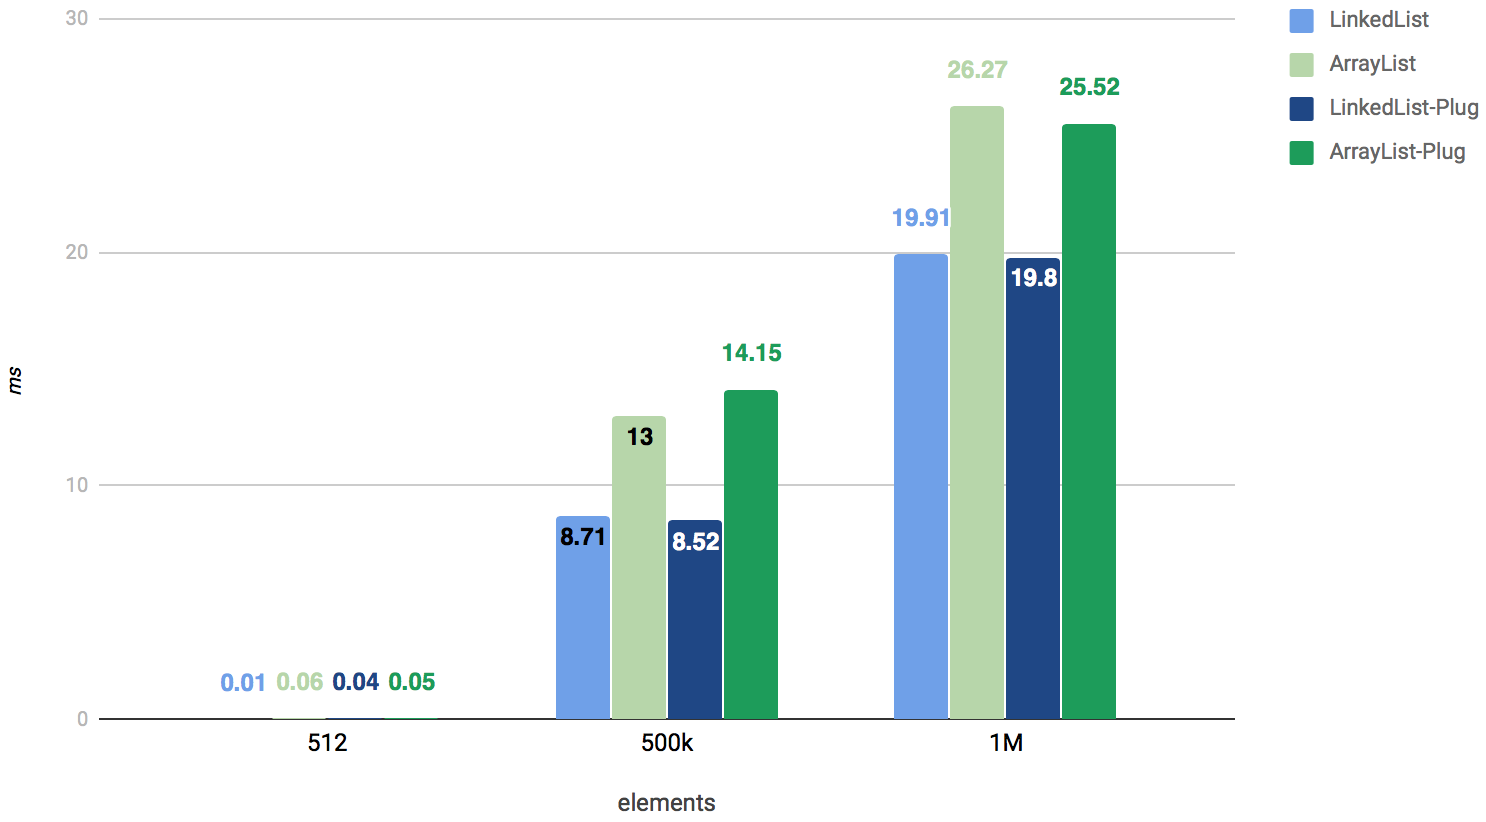
\includegraphics[width=0.9\linewidth]{jayhorn.png}
    \caption{\small Performance of array lists and linked lists both with and without prefetching hints on the Jayhorn benchmark}
    \label{fig:jayhorn}
\end{figure}

Figure \ref{fig:jayhorn} shows the effects of our prefetching hints (in bold) on both linked lists (in blue) and on array lists (in green). In most cases, our plugin has a negligible effect and when traversing an array list of half a million elements, our plugin, in fact, made performance \textit{worse}.

In Figure \ref{fig:cyclistLL}, we consider the performance of linked lists, both iteratively (in blue) and recursively (in green). Once again, the effects of our plugin are represented in bold colors. In this situation, prefetching hints have little to no effect except when recursively traversing a linked list of a million elements, where performance worsens by $19.9\%$.

\begin{figure}[t]
    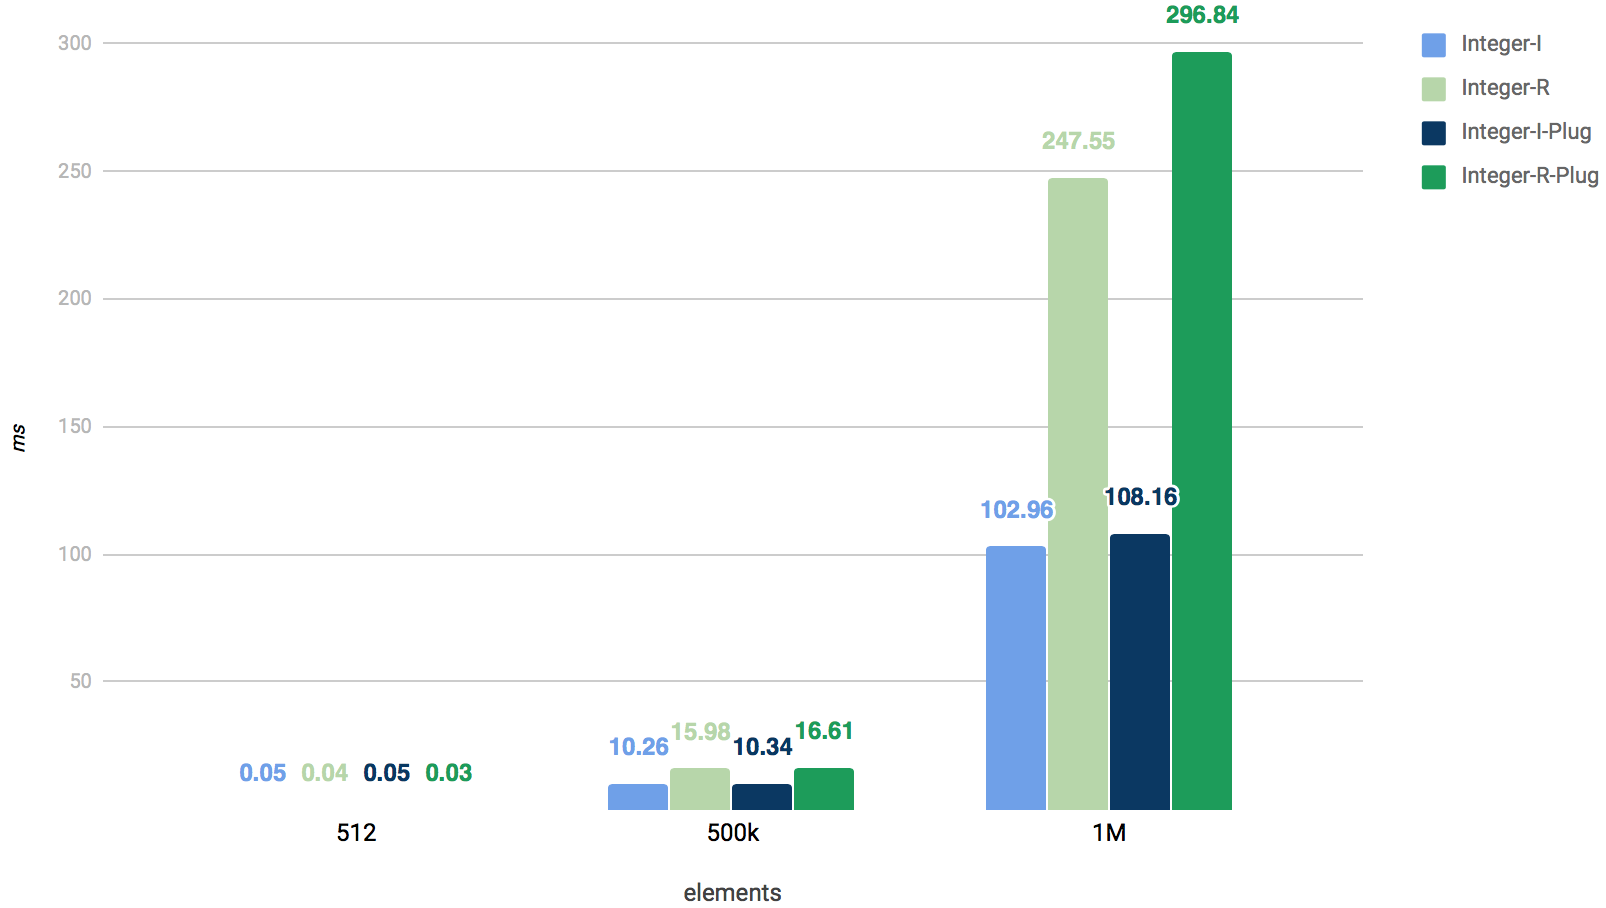
\includegraphics[width=0.9\linewidth]{cyclistLL.png}
    \caption{\small Performance of linked lists both with and without prefetching hints on the Cyclist benchmark}
    \label{fig:cyclistLL}
\end{figure}

Finally, we applied the Cyclist benchmark to array lists, traversed both iteratively (in blue) and recursively (in green): see Figure \ref{fig:cyclistAL}. Here, prefetching degrades performance across the board; performance suffers when traversing linked lists of any meaningful size either iteratively or recursively.

\begin{figure}[b]
    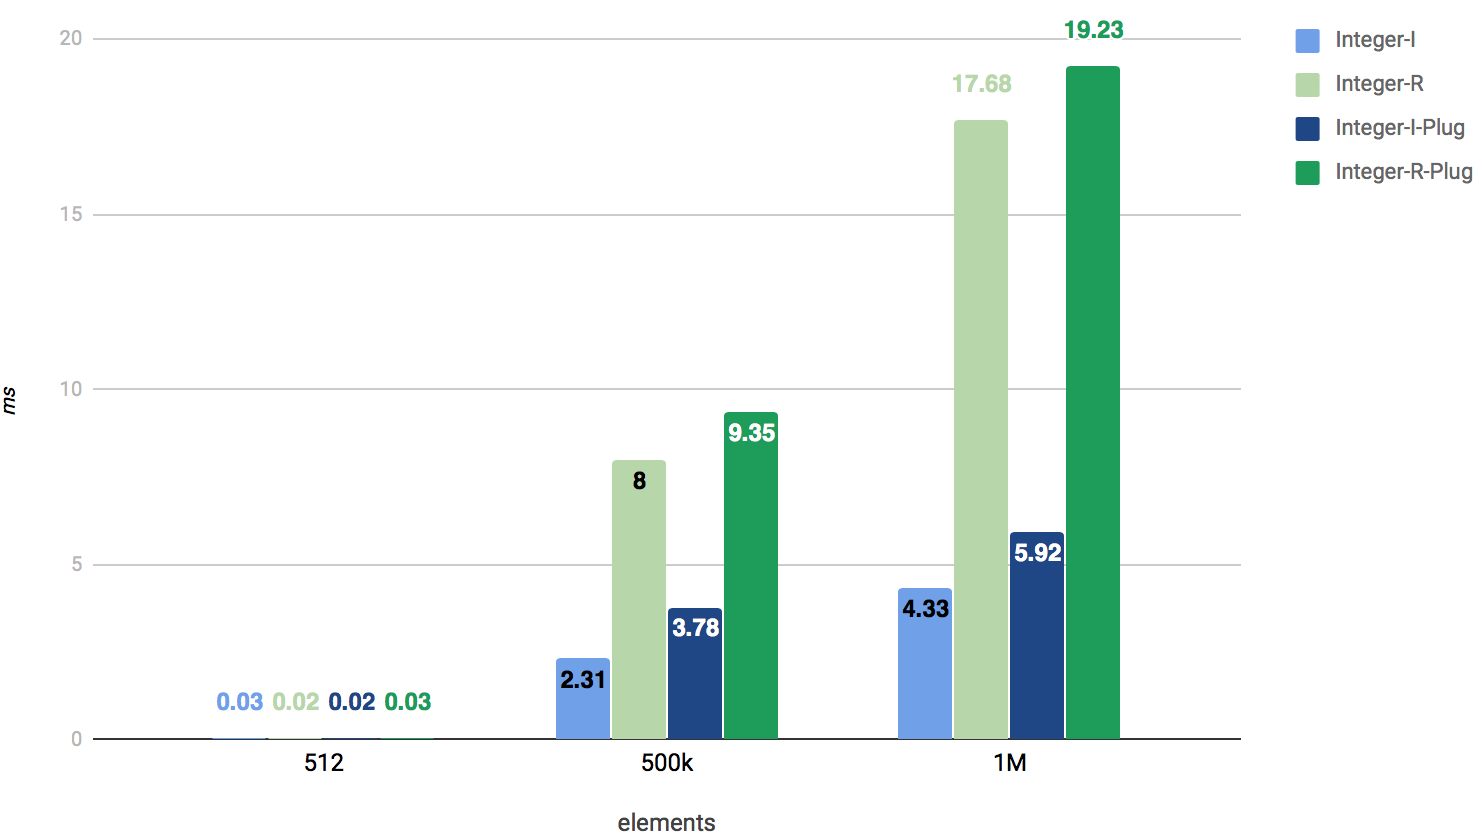
\includegraphics[width=0.9\linewidth]{cyclistAL.png}
    \caption{\small Performance of array lists both with and without prefetching hints on the Cyclist benchmark}
    \label{fig:cyclistAL}
\end{figure}

\subsection{Discussion of Results}

In order to understand these results, we believe it is necessary to consider the Java mechanism of memory management: namely, the fundamental concept that programmers should not need to worry about memory management in Java. Almost all data in Java is encapsulated on objects, which must be dynamically allocated at runtime. This allocation is performed by the garbage collector~\cite{jvmGc}.

The modern JVM employs a hybrid generational mark-and-sweep garbage collector, depending on the size and time at which objects are instantiated. Based on the assumption that the majority of objects are quickly created, used, and released in short spans of time relative to the lifetime of the program, memory is initially allocated within a ``young generation'' area of the heap segment. The young generation is periodically checked for objects that are no longer being used, at which time any surviving objects are moved to the ``old generation'' (which is also periodically collected, potentially using a different algorithm better suited to handle long-lasting objects). The JVM also maintains a third ``permanent generation'' for those objects that will be used over the entire lifetime of the program.

As it is relevant to prefetching, what this means is that the majority of data in Java is not necessarily grouped in memory based on when it is used, but based on when the JVM thinks it is likely to need to be deallocated. Our strategy of approximated prefetching is effectively just a hint to the CPU that data already in cache should stay in cache. Caching, in turn, looks to exploit spatial locality --- and there is no guarantee of spatial locality in Java's memory organization. Thus, our plugin does nothing more than cause the program to block while loading from memory slightly earlier than it would otherwise have done so, and we add the overhead of extra method calls.

Furthermore, we note that since the majority of values in Java are encapsulated within objects, prefetching the elements of an \texttt{ArrayList} or an \texttt{LinkedList} does not truly prefetch the data that will be used by later instructions. Rather, it only prefetches a \textit{reference} to the data. The data itself may still need to be loaded from main memory. In order to realize all the benefits of prefetching, a compiler will need to understand how many pointers to dereference, and, depending on that number, how early to start the process of prefetching. We argue that, at that point, optimization has progressed beyond the point of simple prefetching, and the compiler might as well perform full-fledged loop unrolling or function/method inlining.

\subsection{Prefetching Primitive Arrays}

To test our suspicions regarding the results, we manually added prefetching method calls to the traversals of traditional array containing half a million primitive integers, and compared their runtimes over fifteen trials.

While the JVM standard does not require any particular organization of arrays in memory, in practice, there is little reason not to allocate them as contiguous blocks of memory, so we would expect that standard, language-agnostic caching on the part of the operating system and the architecture would be able to take advantage of locality. Additionally, since arrays can contain primitive values, this setup should be able to avoid the trap of prefetching references instead of actual data values.

\begin{figure}[t]
    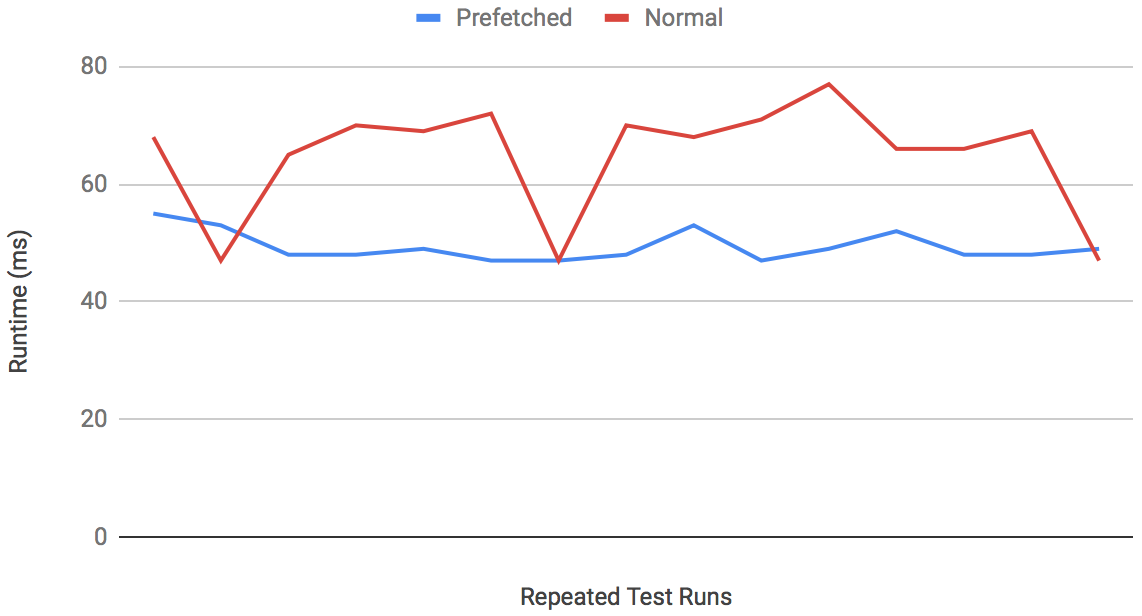
\includegraphics[width=0.9\linewidth]{arrayRecursive.png}
    \caption{\small Performance of traditional arrays traversed recursively, both with and without manually added prefetching hints}
    \label{fig:arrRecursive}
\end{figure}

When this array is traversed recursively, as shown in Figure \ref{fig:arrRecursive}, normal execution times fluctuate, occasionally completing noticeably faster. With the addition of prefetching hints, these runtimes stabilize at those faster speeds. This matches our expectations: at a lower level than the JVM, we sometimes get lucky, and the data we need has been cached for us. By adding statements accessing later array elements, we hint that those elements should remain in cache across the recursive method call.

\begin{figure}[t]
    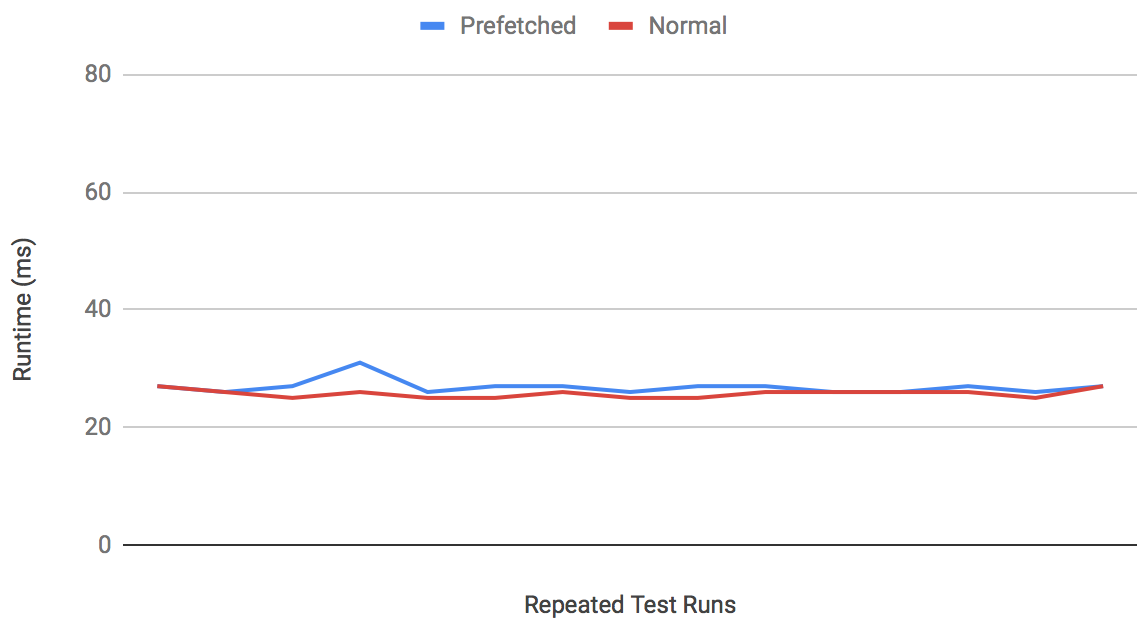
\includegraphics[width=0.9\linewidth]{arrayIterative.png}
    \caption{\small Performance of traditional arrays traversed iteratively, both with and without manually added prefetching hints}
    \label{fig:arrIterative}
\end{figure}

On the other hand, when that same operation is performed iteratively, seen in Figure \ref{fig:arrIterative}, runtime is consistent both with and without any prefetching statements. This, too, matches our expectations: without the intervening recursive method call, there simply aren't any operations that could cause the array elements to be removed from cache; no hints are necessary.


\section{Conclusions}

We have implemented a plugin for the reference Java compiler that attempts to approximate the effects of prefetching, despite the fact that the JVM provides no support for that optimization at the compiler level. We have theorized that, due to the manner in which memory is managed by the JVM, prefetching would have little effect; our theory superficially appears to be confirmed by the Java development team's recent decision to remove any support from prefetching from their experimental libraries. In keeping with that theory, we have shown that such a plugin provides no improvement in the runtime of Java programs that traverse large list structures.


\section{Future Work and Source Code}

While we do not believe there is much performance to be gained through compiler-driven prefetching of sequential data structures in Java, our source code can be found at \texttt{\url{https://github.com/cesiu/JavaListPrefetcher}}.


\bibliography{references}
\bibliographystyle{ieeetr}


\end{document}
